\documentclass{article}

\usepackage{graphicx}
\usepackage{amsmath}

\title{A Trading Algorithm}

\author{Babak Emami}

\date{\today}

\begin{document}
\maketitle

\section{Introduction}\label{introduction}

Here, I mention the trading strategies I undestand from the trading
code by Abbas, as well what we discessed verbally. A trading algorithm
is then outlined which is based on a combination of these strategies.

\section{Strategies}\label{section:abbas-strategies}

\subsection{Mean Absolute Deviation Minimization}\label{section:mad}

Given a set of securties, the Mean Absolute Deviation (MAD) is
minimized to obtain portfolio weights, that is percentage of asset
allocations. The MAD of a signal $x(t)$ (as a function
of time $t$), $F_{MAD}$ is defined as,

\begin{equation}\label{eqn:mad}
F_{MAD}(x(t)) = \frac{1}{N_{hist}}\sum_{t=t_{curr}}^{t_{curr}-N_{hist}+1} |x(t)-\bar{x}|
\end{equation}

where $t_{curr}$ is current time, $N_{hist}$ is number of historical
data points used, and $\bar{x}$ is the avergae of the signal in the
period $t_{curr}-N_{hist}+1$ to $t_{curr}$.

Let us have a portfolio with $n$ assets $x_{i}(t)$ where $i = 1,
...,n$, with weights $w_{i}$, where positive and negative weights are
long and short positions, respectively and $\sum_{i=1}^{n} |w_{i}|
= 1$. The portfolio MAD is the given by,

\begin{equation}\label{eqn:mad}
F_{MAD}(\vec{x}(t),\vec{w}) = \frac{1}{N_{hist}}\sum_{t=t_{curr}}^{t_{curr}-N_{hist}+1}
|\sum_{i=1}^{n} w_{i} (x_{i}(t)-\bar{x_{i}})|
\end{equation}

Here on, we refer to this strategy as MAD.

\subsection{Moving Average Convergence Divergence}\label{section:macd}

Mean Average Convergence Divergence (MACD) is used to calculate short
term acceleration of a security and as such helps with making a
decision to take a long or short position on a security. MACD of a
signal $x(t)$ is defined as,

\begin{equation}\label{eqn:macd}
F_{MACD}^{(f,s)}(x)|_{t_{curr}} = E^{f}(x)|_{t_{curr}} -
E^{s}(x)|_{t_{curr}}
\end{equation}

where $E^{p}$ represents exponential moving average with respect to a
period $p$, and $f$ and $s$ are fast and slow periods,
respectively. The signal $x(t)$ has a positive/negative acceleration
at $t=t_{curr}$ if $F_{MACD}^{(f,s)}(x)|_{t_{curr}}$ is
greater/smaller than $E^{r}(F_{MACD}^{(f,s)}(x))|_{t_{curr}}$, where
$r$ is called the signal period. The starndard values for fast, slow,
and signal periods are 12, 26, and 9 days, respectively. One should
long/short when acceleration becomes positive/negative. In fact, one
can check the sign of both $F_{MACD}^{(f,s)}(x)|_{t_{curr}}$ and
$F_{MACD}^{(f,s)}(x)|_{t_{curr}}-E^{r}(F_{MACD}^{(f,s)}(x))|_{t_{curr}}$
as they represent velocity and acceleration signs, respectively. The
number of historical times used to calculate MACD should be at least
$s$ + $r$ ($N_{hist} > s + r$).

Here on, we refer to this strategy as MACD.

\subsection{Mean and Standard Deviation of Price}\label{section:msdp}

Another strategy to make a decision about taking long or short
positions is to look at the mean and standard deviation of price. For
a given securty price $p(t)$, we can define,

\begin{equation}\label{eqn:mean-price}
\bar{p} = \frac{1}{N_{hist}} \sum_{t=t_{curr}}^{t_{curr}-N_{hist}+1} p(t)
\end{equation}

and,

\begin{equation}\label{eqn:std-price}
\sigma^{2}(p) = \frac{1}{N_{hist}} \sum_{t=t_{curr}}^{t_{curr}-N_{hist}+1} (p(t) - \bar{p} )^{2}
\end{equation}

where $\bar{p}$ and $\sigma(p)$ are mean and standard deviation of
price $p(t)$, respectively.

If $p(t_{curr}) < \bar{p} - \zeta_{price} \sigma(p)$, then the asset
is under-priced and its price will likely increase. So we should take
a long position. Similarly, when $p(t_{curr}) > \bar{p} +
\zeta_{price} \sigma(p)$, then the asset is over-valued and its price
will likey decrease, and thus one should take a short position on that
asset. We start with $\zeta_{price}$ = 1.75, and $N_{hist}$ = 20 days.

Here on, we refer to this strategy as MSDP.

\subsection{Mean and Standard Deviation of Volume}\label{section:msdv}

This is similar to the above strategy, but we look at the traded
volume rather than price. In other words, if $v(t_{curr}) < \bar{v} -
\zeta_{volume} \sigma(v)$, then the asset is under-traded and its
value will likely increase. So we should take a long
position. Similarly, when $v(t_{curr}) > \bar{v} + \zeta_{volume}
\sigma(v)$, then the asset is over-traded and its value will likey
decrease, and thus one should take a short position on that asset. A
standard value for $\zeta_{volume}$ is 1.75.

Here on, we refer to this strategy as MSDV.

\subsection{Relative strengths}\label{section:rls}

Another strategy is to look at the relatice strength (value ratio) of
the asset price with respect to a standard benchmark such as $SPY$. We
can look at the historical strength ratios and calculate the mean and
standard deviation. If a certain asset is being traded well outside of
its histrical relative strength, that often implies the asset is under
or over valued and so its value is likely to increse or decrease,
respectively. As such, we take a long position if $R(t_{curr}) <
\bar{R} - \zeta_{rls} \sigma(R)$ and a short position when
$R(t_{curr}) > \bar{R} + \zeta_{rls} \sigma(R)$, where $R(t)$ is
relative strength of an asset at time t.

Here on, we refer to this strategy as RLS.

\section{A Trading Algorithm}\label{section:algorithm}

Out of the five above-mentioned approaches, one, namely MAD, can be
used to determine asset allocation and the other four can be used to
determine whether one should long or short on an asset. 

One approach is to minmize MAD to obtain portfolio weights (asset
allocations) and a weighted average of the position recommended by
MACD, MSDP, MSDV, and RLS as constraints.

To do a weighted average of MACD, MSDP, MSDV, and RLS predictions, we
can give a weight $W_{S}$ to each strategy such that $W_{S} \in [0,1]$
and $\sum_{S=1}^{4} W_{S}$ = 1. Then we can determine the probability
of a price increase,$P^{u}$, as

\begin{equation}\label{eqn:increase-prob}
P^{u} = \sum_{S=1}^{4} W_{S} \eta_{S}^{u} 
\end{equation}

where $\eta_{S}^{u}$ = 1 if the strategy $S$ predicts an upward price
change, and 0 otherwise. Similarly, we can determine the probability
of a price decrease,

\begin{equation}\label{eqn:increase-prob}
P^{d} = \sum_{S=1}^{4} W_{S} \eta_{S}^{d} 
\end{equation}

where $\eta_{S}^{d}$ = 1 if the strategy $S$ predicts a downward price
change, and 0 otherwise.

We will start with $W_{MACD}$ = 0.6, $W_{MSDP}$ = 0.1, $W_{MSDV}$ =
0.1, $W_{RLS}$ = 0.2.

If the probability of a price to increase or decrease is more than a
certain threshold, then we go long or short on it.

\section{Summary}

In summary, the following constraint optimization problm should be
solved,

\begin{equation}\label{eqn:summary}
\min_{w_{i}} \sum_{t=t_{curr}}^{t_{curr}-N_{hist}+1} |\sum_{i=1}^{n} w_{i} (x_{i}(t)-\bar{x_{i}})|
\end{equation}

subject to $P^{u}_{i} \geq P^{threshold} \Rightarrow w_{i} \geq 0$ and
$P^{d}_{i} \geq P^{threshold} \Rightarrow w_{i} \leq 0$.

\section{Timing of Trades}\label{section:timing}

The are two concepts with respect to the timing of trades, namely
holding period and portfolio adjustment frequency. We start trading a
certain set of assets at some point in time and close all positions
after the holding period. During this time, the portfolio weights are
adjusted at a certain frequency. Let us refer to holding period and
adjustment frequency as timing pair. Four sets of timing pairs are
recommended,

1) A holding period of one day and adjustments every 45 minutes. All
positions are closed by the end of the day.

2) A holding period of 5 business days, and daily adjustments.

3) A holding period of a month, and daily adjustments.

4) A holding period of 3 months and adjustments every 3 or 4 days.

When trades are done once a day or at an even slower cadence, it is
recommended that we do all transactions between 3 and 4 pm ET.

\section{Seasonality}\label{section:seasonality}

It seems that a seasonality exists in the
market. Figure~\ref{fig:seasonality} shows the average of S\&P500
index as a function of calendar months. When one trades on one or 3
months holding periods, the seasonality should be taken into account.

\begin{figure}\label{fig:seasonality}
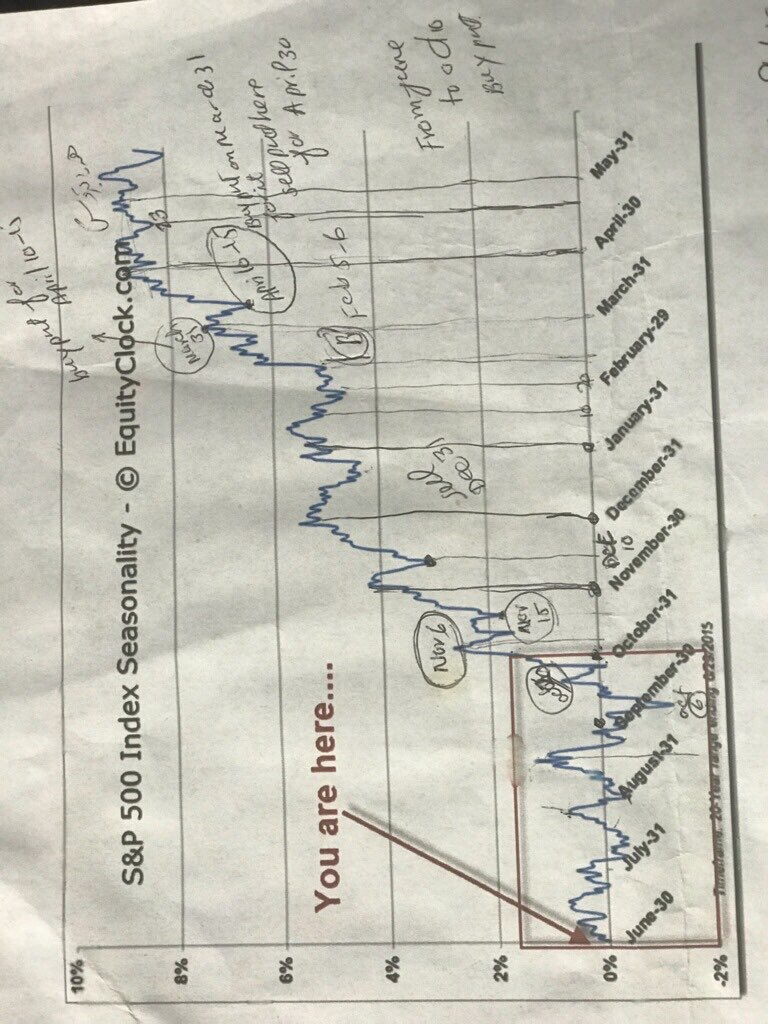
\includegraphics[width = \textwidth, angle = -90 ]{figures/seasonality.JPG}
\caption{Seasonality of S\&P500 index.}
\end{figure}

\end{document}

